\chapter{Features' importance}

After having determined the most performant algorithm, which is Random Forest, it is time to go further and analyse which features impact the results of classification the most. The focus will be especially on false predictions. In order to do that, six different tools for feature analysis will be discussed and compared.

\section{Result's interpreters' comparison}

The six mentioned tools are: LIME \cite{lime}, ELI5 \cite{mikhail_korobov_eli5_nodate}, YellowBrick \cite{bengfort_yellowbrick_2018}, Treeinterpreter \cite{ando_saabas_treeinterpreter_nodate}, dtreeviz \cite{terence_parr_dtreeviz_nodate} and export\_graphviz tool from scikit-learn, where the last three ones are designed for Decision Tree and Random Forest classifiers.

\subsection{LIME} 
LIME (Local Interpretable Model-agnostic Explanations) is a tool that is used to explain the behaviour of machine learning classifiers. It supports, as for this day, only the explanation of individual predictions for any scikit-learn classifier or regressor. This explanation consist in a list of features (and more precisely decision nodes composed of feature name and a numeric condition) ordered by their relative importance for a particular prediction. This list can be shown is a raw mode (as a python list) or in a visual form (pyplot figure, jupyter notebook or html file).

In order to class the features according to their importance, LIME approximates the model by an interpretable one, created based on perturbing the features of the examined instance. More the perturbed instances are similar to the examined instance, higher is the weight of the perturbed feature. This approximation process is called explanation and is described using the following equation:

\begin{equation}
    \xi(x) = \operatorname*{argmin}_{g \in G} \mathcal{L}(f, g, \pi_x) + \Omega(g)\quad\cite{lime},
\end{equation}

\noindent where $g$ is the explanation model from the set of interpretable models $G$, $f$ is the probability that the sample $x$ corresponds to a certain class, $\pi_x$ is the distance between an instance $z$ and the sample~$x$. $\mathcal{L}(f, g, \pi_x)$ describes to which extent $g$ is unfaithful in the approximation of $f$ in the neighbourhood defined by $\pi_x$, while $\Omega(g)$ describes the complexity of the explanation (for example the depth of the tree if $f$ is a decision tree). The goal of the explanation is to find the most faithful approximation of $f$ taking into consideration the neighbourhood $\pi_x$.

To better illustrate the algorithm, let the pigeon image in figure \ref{fig:limepigeon} be considered as a sample used in a classification problem based on a classifier noted \textit{f}. The image can be divided into several regions, like it is shown in figure \ref{fig:limediv}, each region corresponds to a feature.

\begin{minipage}{.45\textwidth}
    \begin{figure}[H]
        \centering
        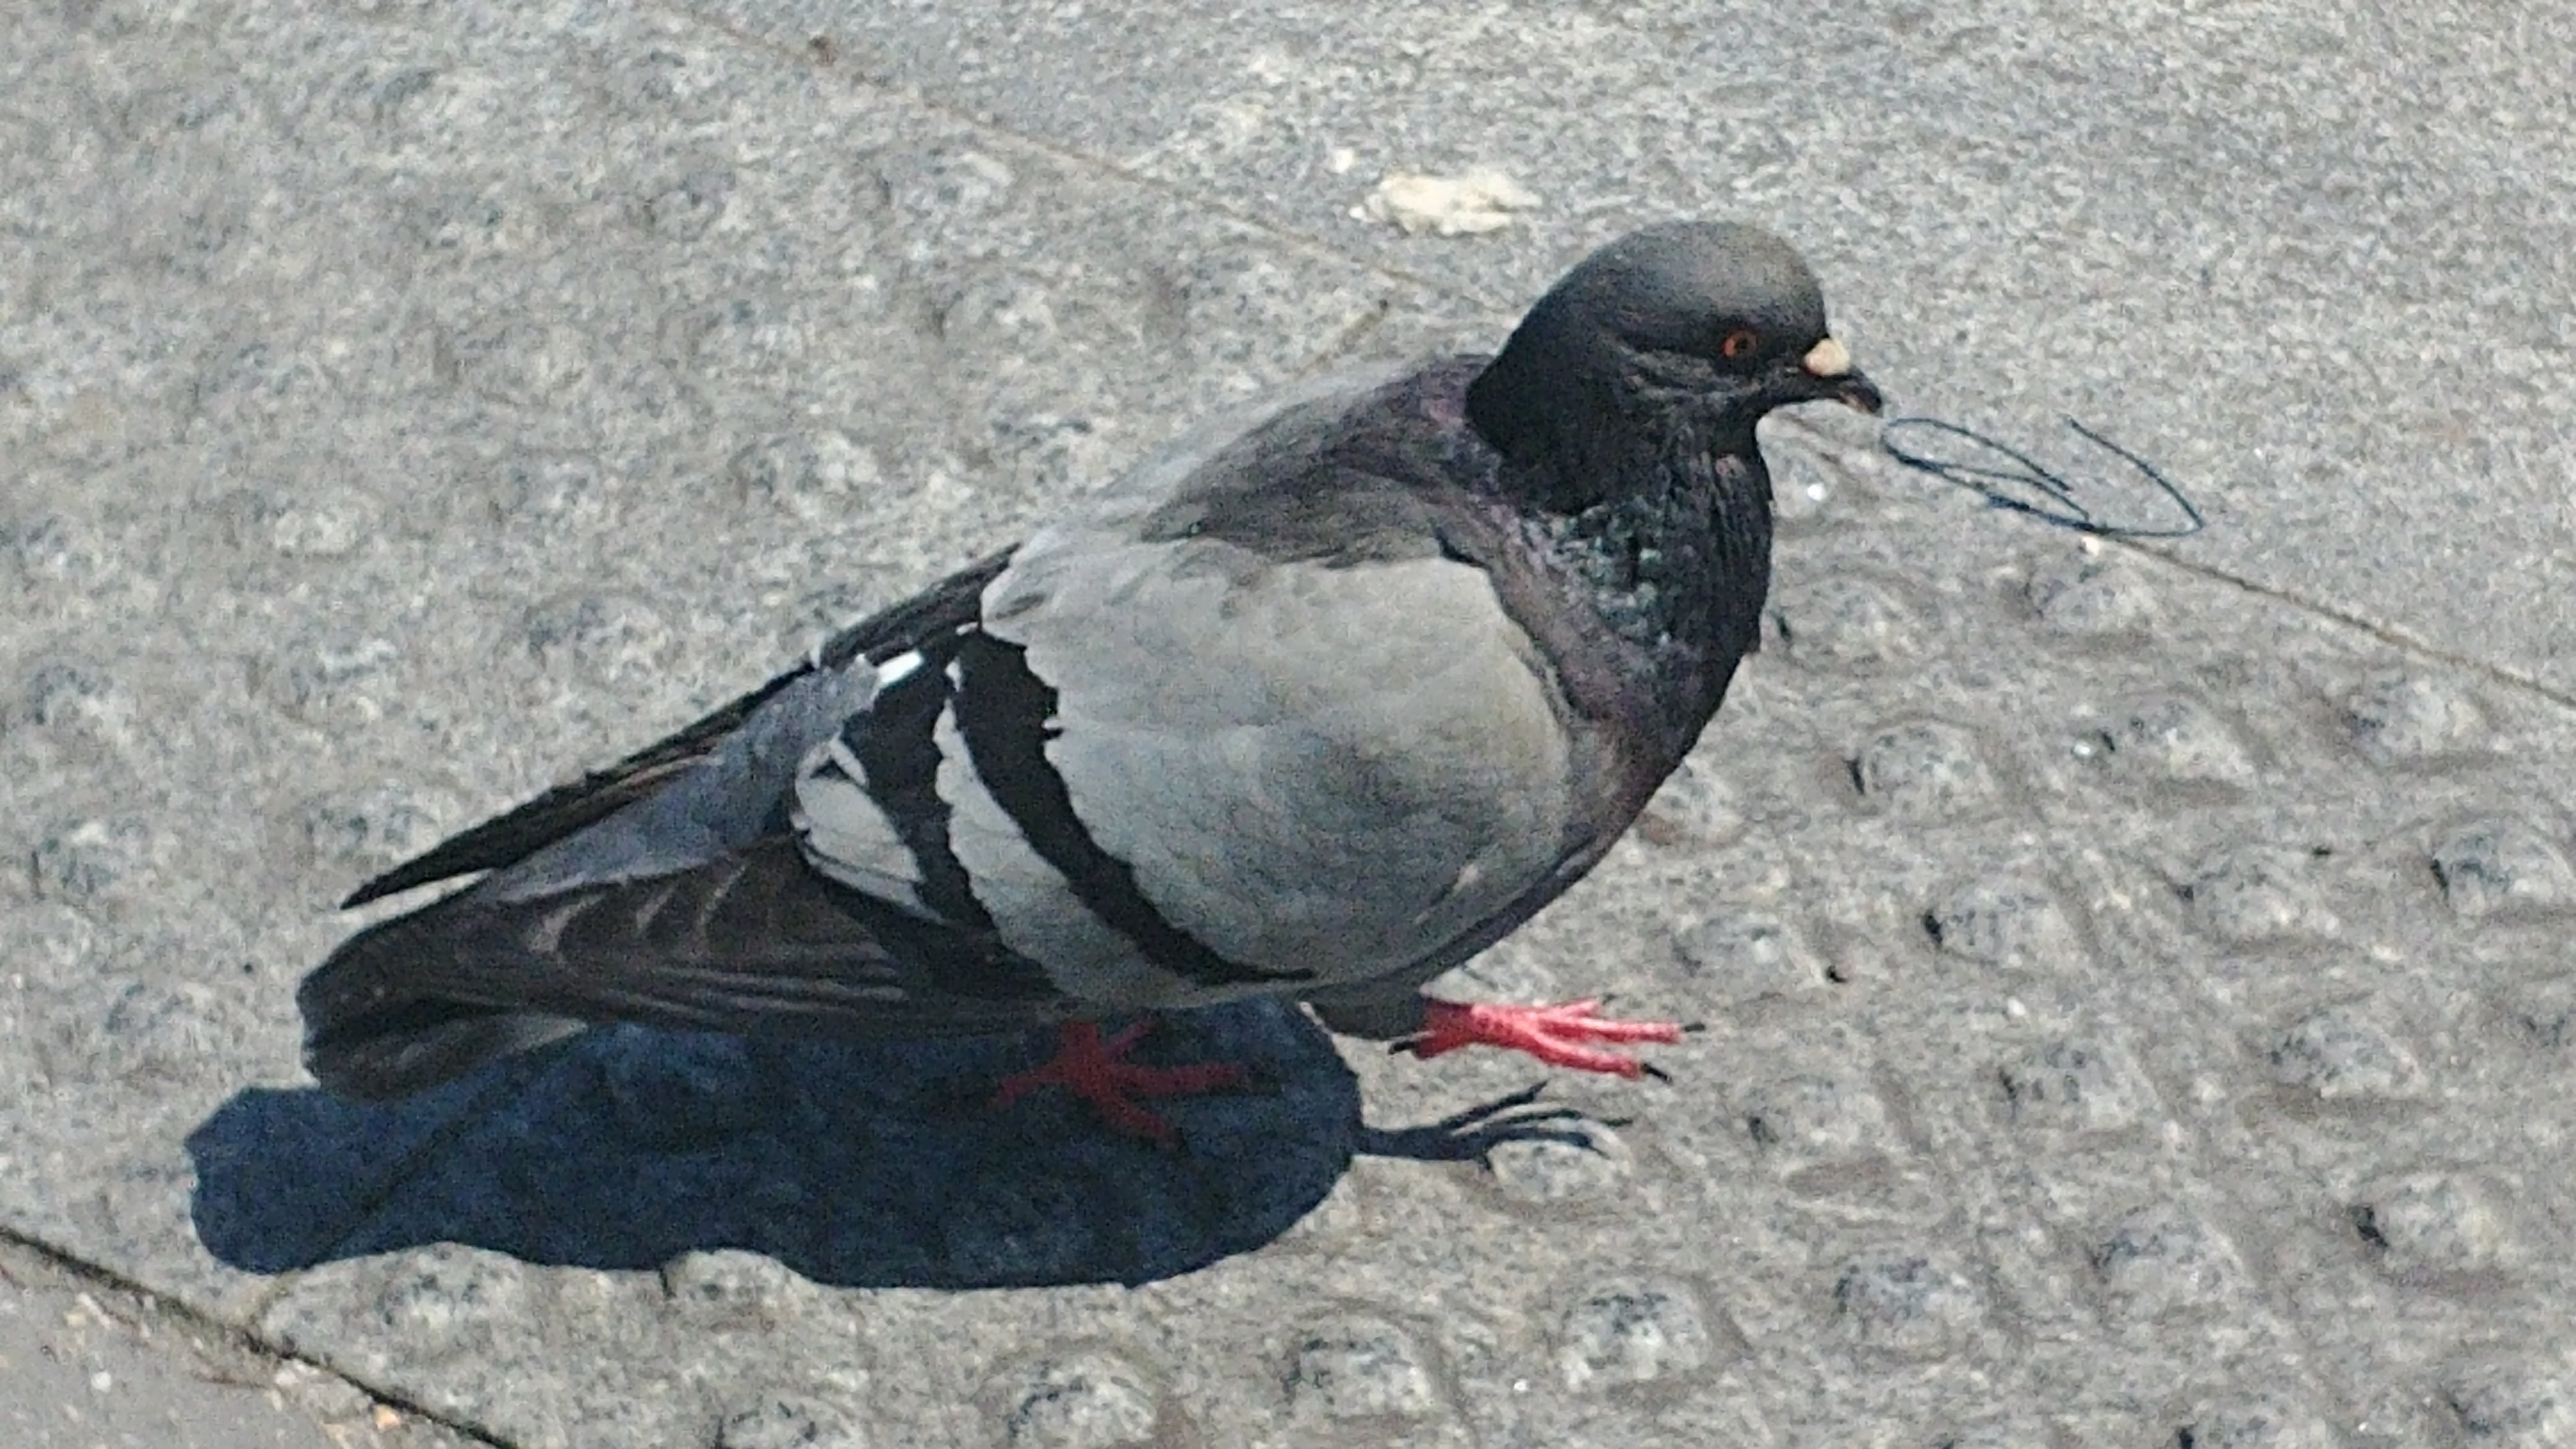
\includegraphics[width=\linewidth]{images/lime/pigeon}
        \caption{Pigeon}
        \label{fig:limepigeon}
    \end{figure}
\end{minipage}
\begin{minipage}{.45\textwidth}
    \begin{figure}[H]
        \centering
        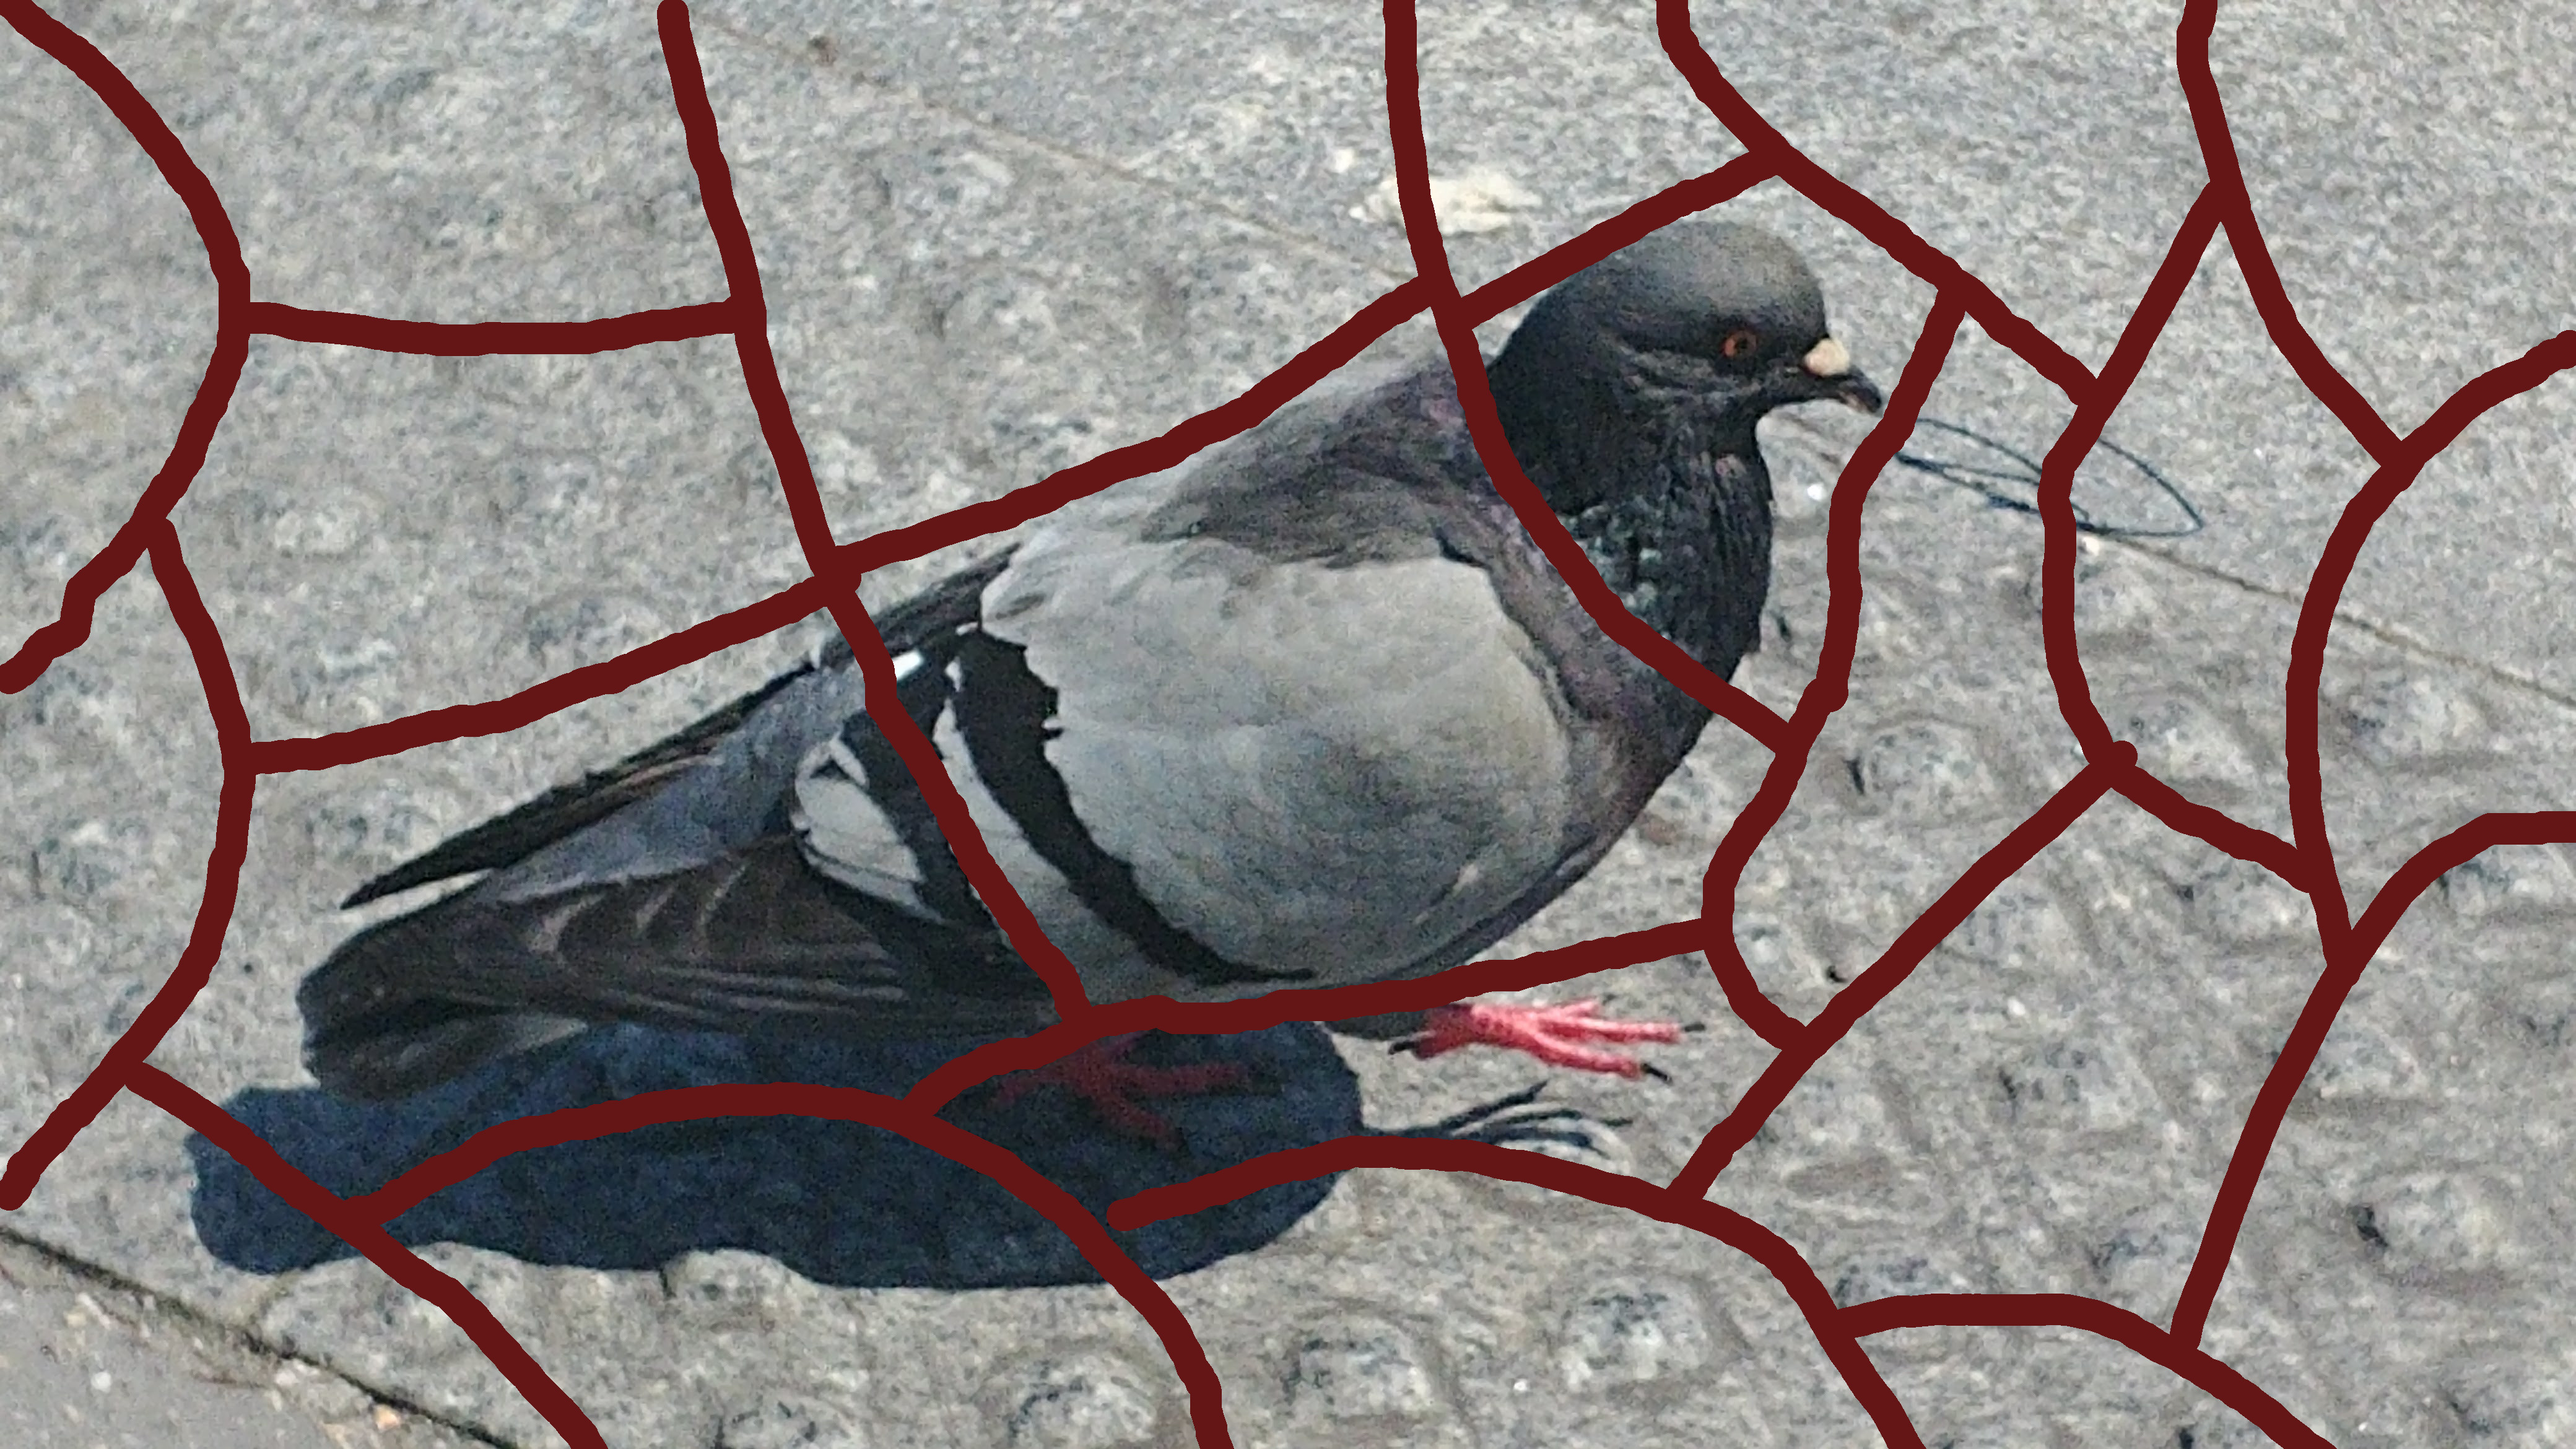
\includegraphics[width=\linewidth]{images/lime/grid}
        \caption{Image grid}
        \label{fig:limediv}
    \end{figure}
\end{minipage}
\vspace{0.5cm}

In the next step, a new dataset is created by modifying the features. In the case of the pigeon image some regions can be simply greyed out like it is shown in figure \ref{fig:limegrey}. For each of these regions the probability if it represents a pigeon or not is calculated using the classifier \textit{f}.

\begin{figure}[H]
    \centering
    \begin{subfigure}[t]{0.32\linewidth}
        \centering
        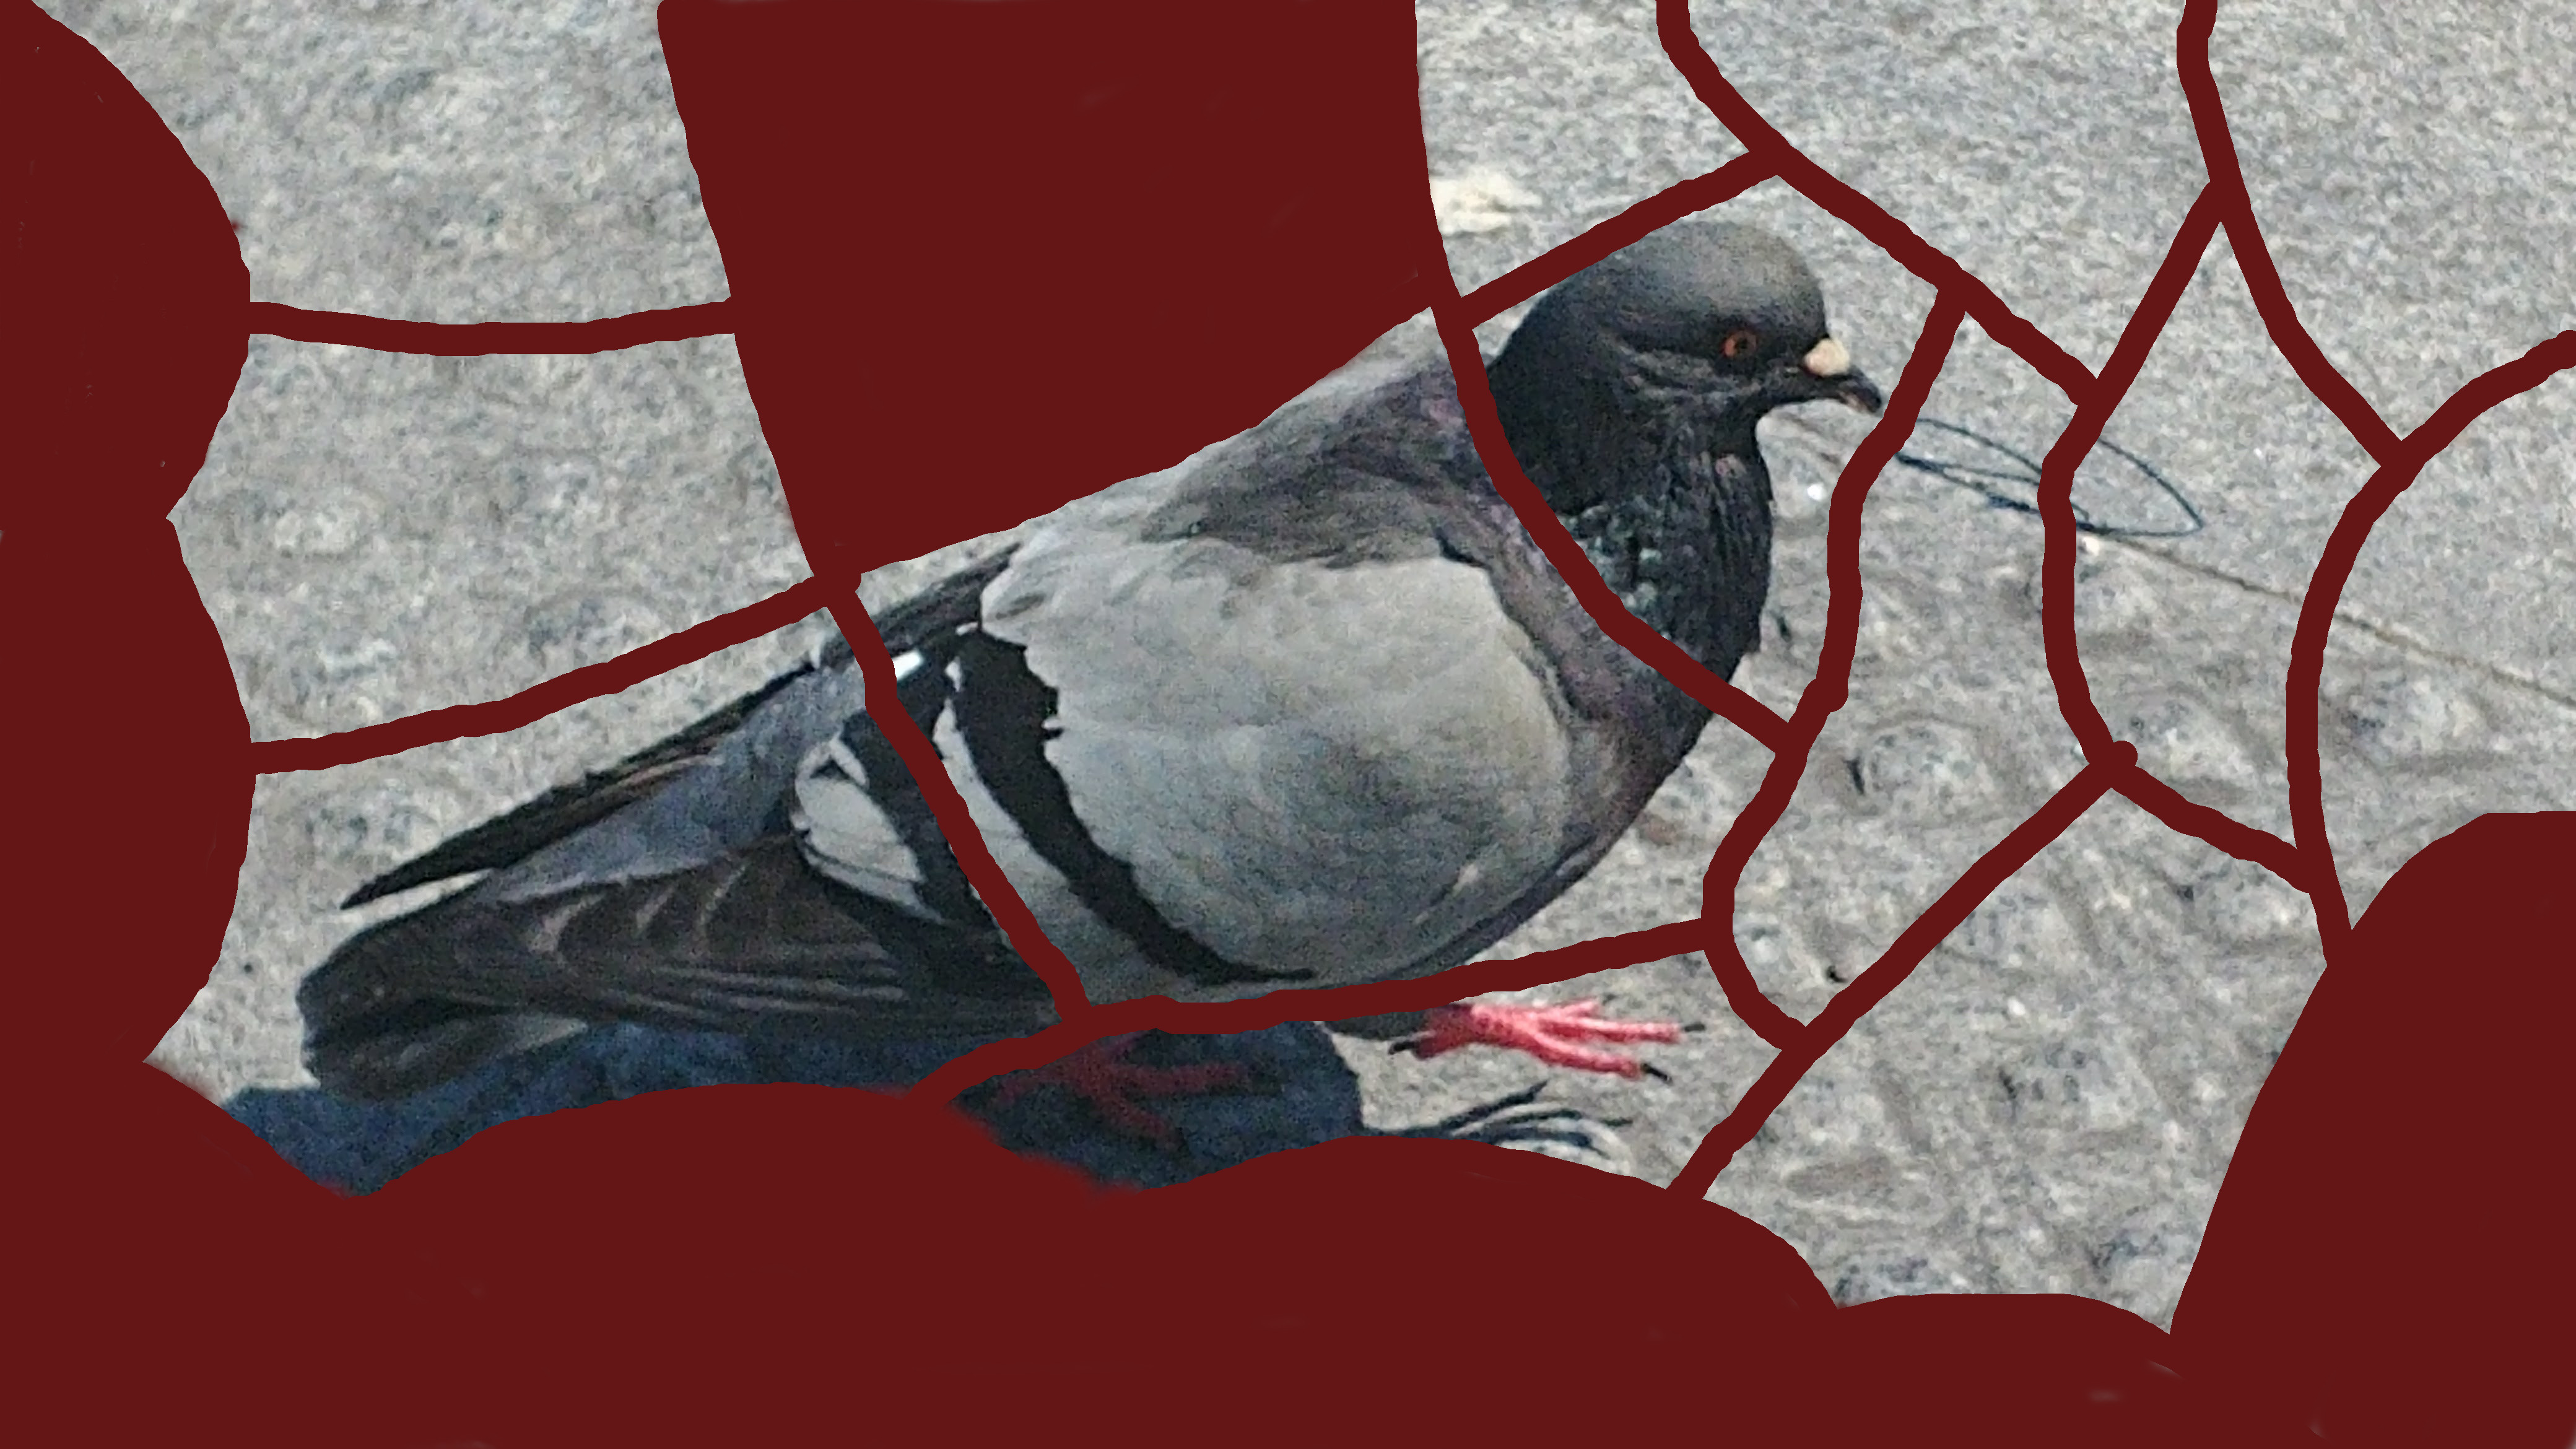
\includegraphics[width=\linewidth]{images/lime/pert1}
        \caption{Perturbation 1}
    \end{subfigure}
    \begin{subfigure}[t]{0.32\linewidth}
        \centering
        
\includegraphics[width=\linewidth]{images/lime/pert2}
        \caption{Perturbation 2}
    \end{subfigure}
    \begin{subfigure}[t]{0.32\linewidth}
        \centering
        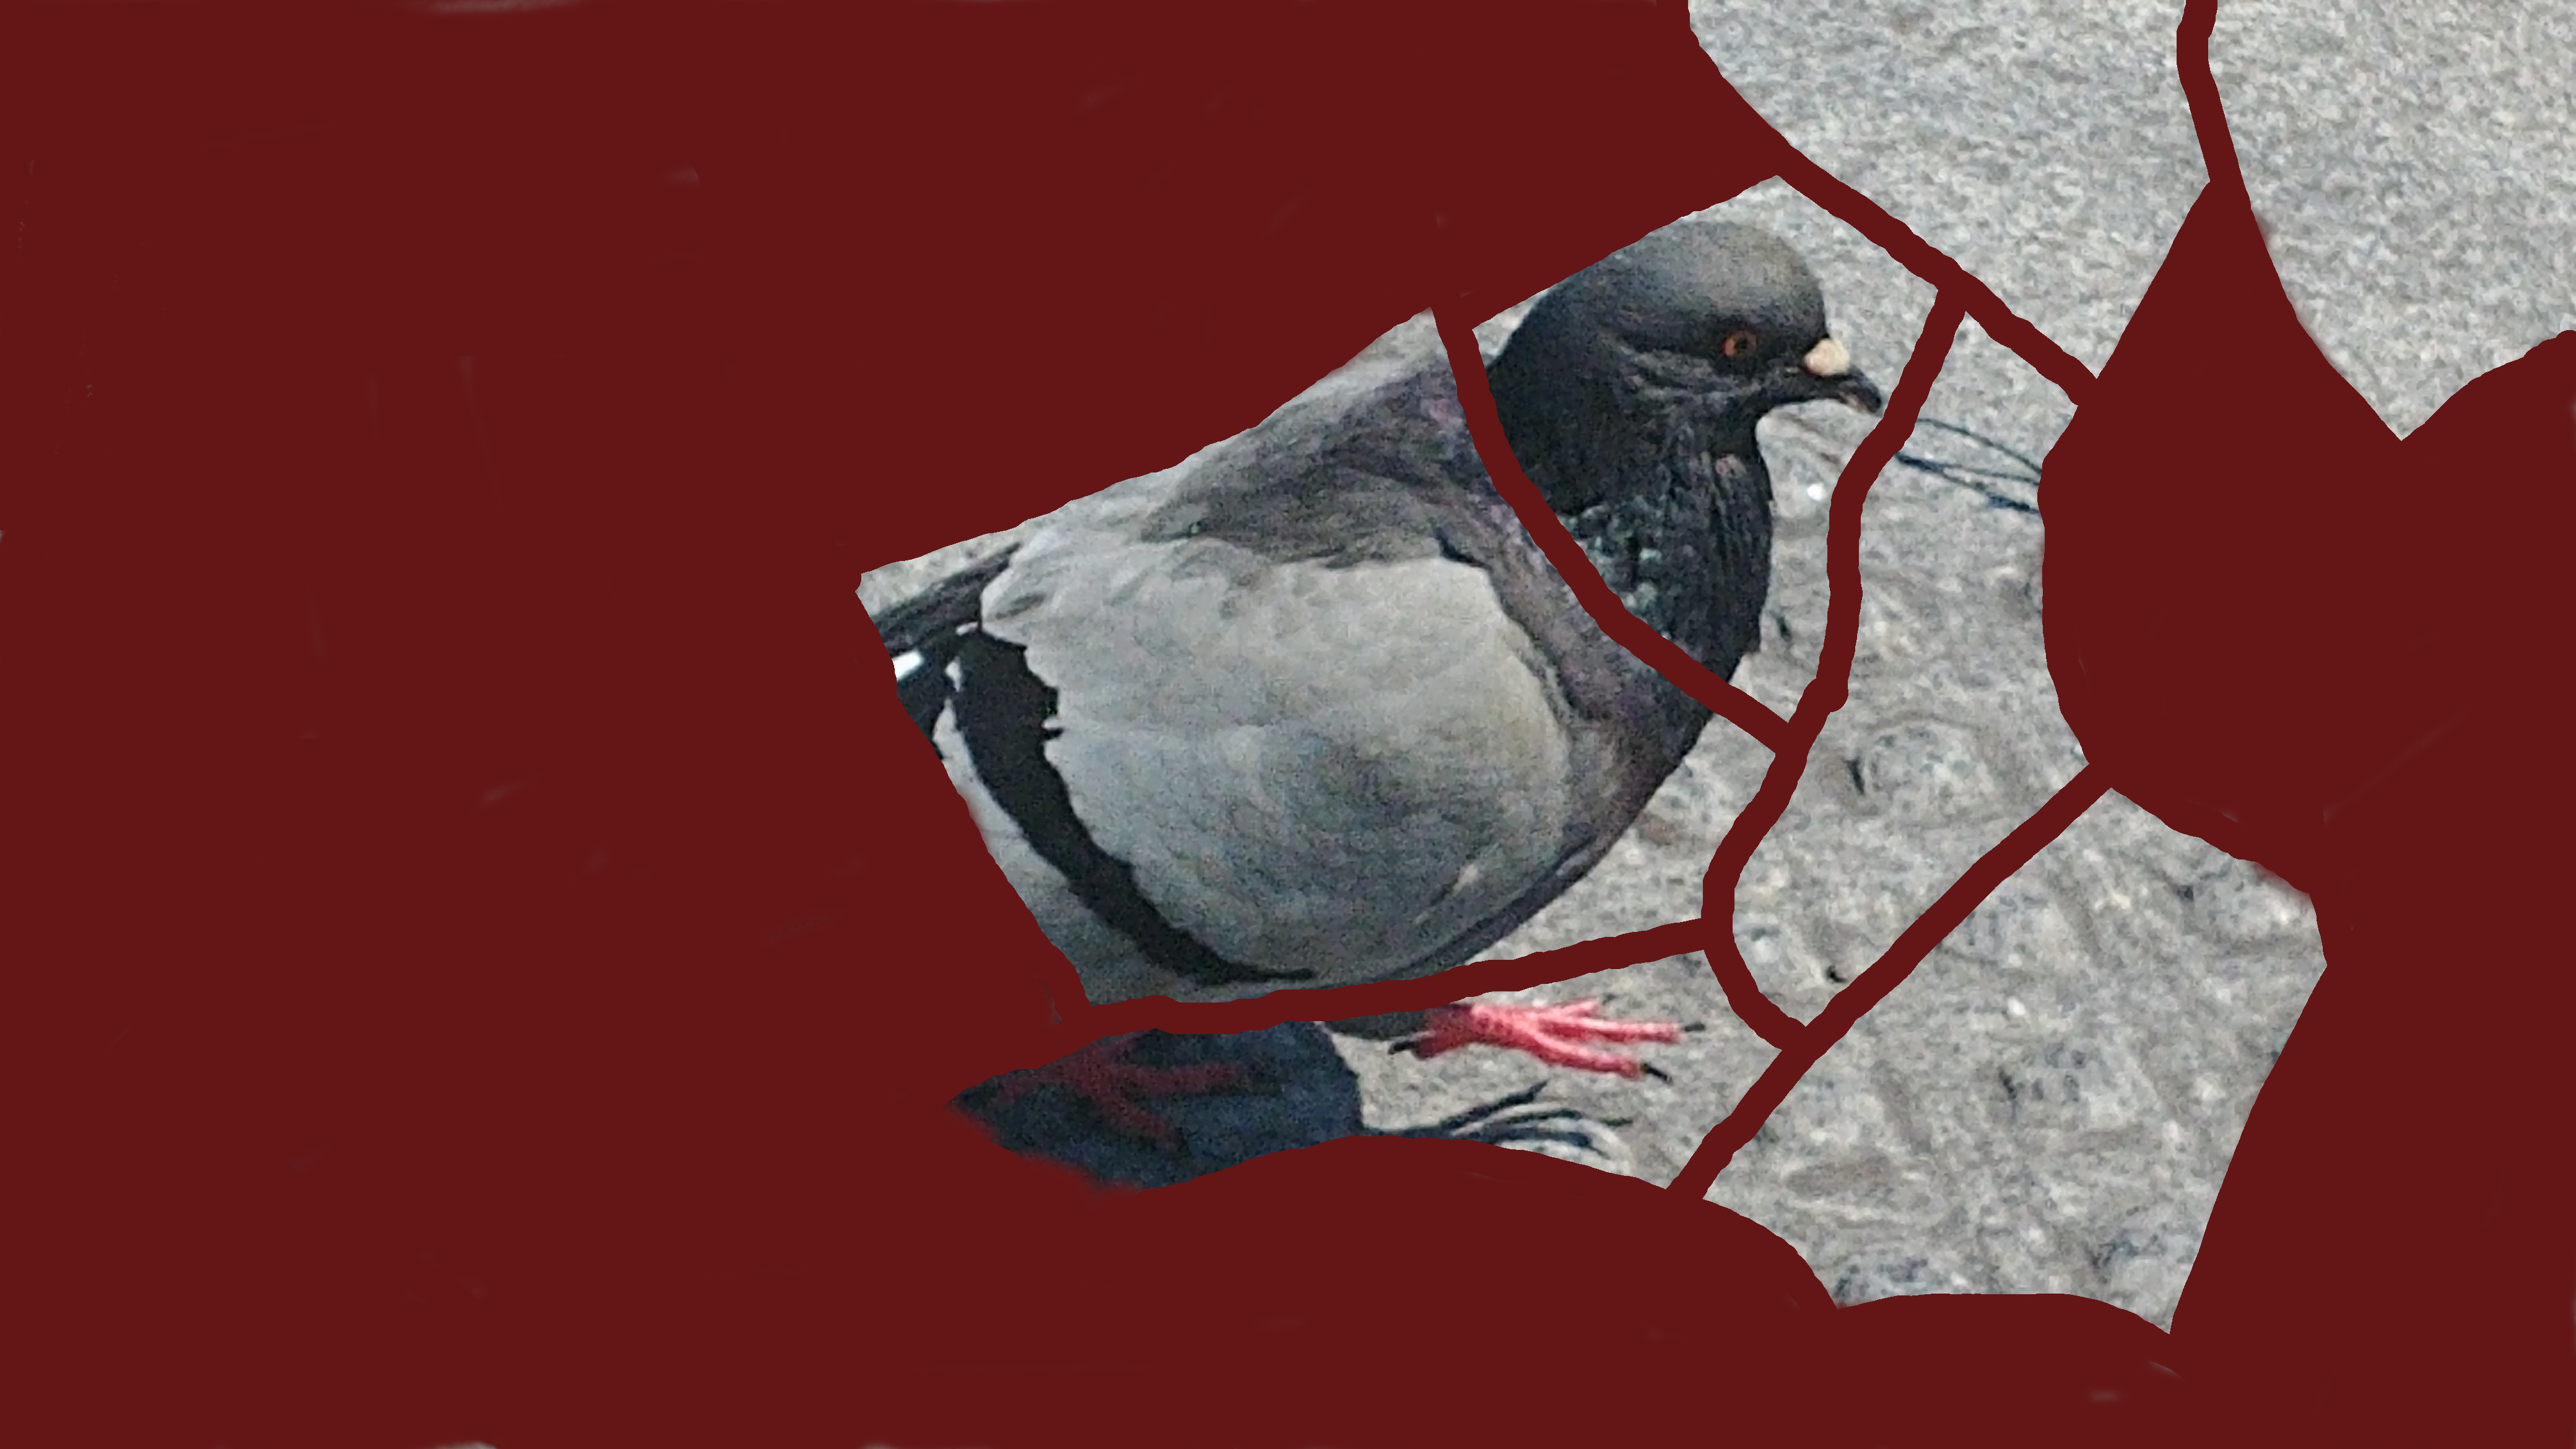
\includegraphics[width=\linewidth]{images/lime/pert3}
        \caption{Perturbation 3}
    \end{subfigure}
    \caption{Greyed-out images forming a new dataset}
    \label{fig:limegrey}
\end{figure}

Using this data it is possible to determine the importance of regions/features of this particular sample. This importance is local and has a meaning only in relation to the sample image from figure~\ref{fig:limepigeon}. 

\subsection{ELI5}
ELI5 (Explain like I am a 5-year old) is a tool, in form of a Python package, used to debug machine learning classifiers and explain their predictions. It supports multiple machine learning frameworks, including scikit-learn. It can be used to explain how the model works both locally for one prediction and globally for the whole model. The output can take several forms just like in LIME case.

For white-box models, ELI5 works as an extension of scikit-learn and it is capable to extract the weights of model's features for different classes. In addition to that it can show the weights that contributed in a particular prediction. It is done by removing particular features and checking how the accuracy of the classifier was altered. On the other hand, for black-box models, this tool integrates a modified version of LIME, supporting more machine learning frameworks, and a permutation importance method, which checks how the model's accuracy decreases when removing one of the features and on this basis determines the importance of the features.

\subsection{YellowBrick}
YellowBrick is another Python package, which is an extension of scikit-learn framework. It is meant to give global interpretation of the analysed model on different levels. It is possible not only to visualize features importances calculated directly by scikit-learn, but also to give a classification report (accuracy, recall, precision, f-measure), plot a confusion matrix, a ROC curve and much more. In addition to all that, YellowBrick comes with a tool for determination of correlation between features in the dataset.

\subsection{Treeinterpreter}
Treeinterpreter is a simple Python package that works with scikit-learn trees and random forest classifiers. It's only usage consists in decomposing the obtained prediction into bias and contributions of different features. The output is given in the form of a numpy array.

\subsection{scikit-learn export\_graphviz}
export\_graphviz is a scikit-learn embedded function that enables the user to visualize a decision tree with all the branches and save it into Graphviz\footnote{a set of tools for diagram creation using graphs.} format, that can be converted into a vector graphic. It is possible also to visualize decision trees composing random forest model in scikit-learn, since the possibility to extract particular decision trees when using this framework. However the interpretability of results for random forest classifier can be hard.

\subsection{dtreeviz}
dtreeviz is a more advanced version of export\_graphviz available in scikit-learn. For every leaf in the tree it can show a histogram indicating the influence of feature's value on class selection. In addition to that, dtreeviz enables the user to show the path of a particular prediction. The result is saved in the form of a svg vector graphic. 

% \begin{figure}[tb]
%     \centering
%     \makebox[\textwidth]{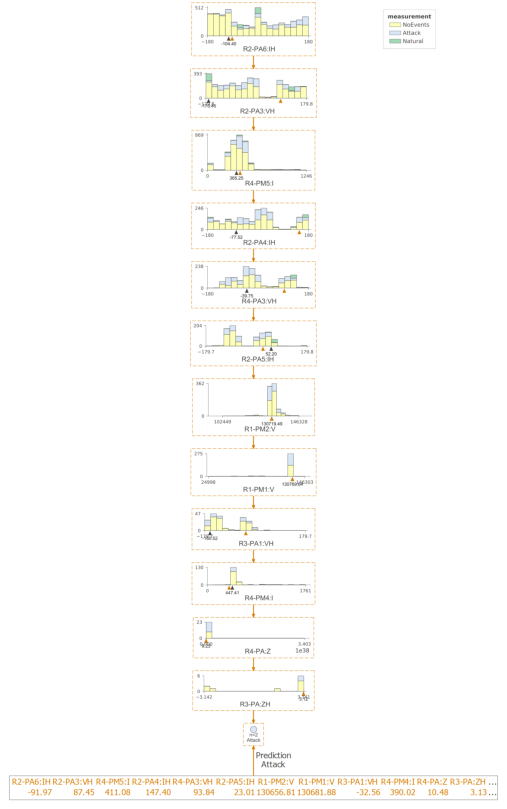
\includegraphics[width=.9\paperwidth, height=.9\textheight]{images/dtreeviz}}
%     \caption{dtreeviz's visualisation of the prediction path for Natural event mispredicted as Attack}
%     \label{fig:dtreeviz}
% \end{figure}



\subsection{Summary}
It can be concluded that ELI5 is the most versatile package compared to others, especially because it enables both global and local interpretations and does not limit its support to scikit-learn, plus it has LIME integrated in it. YellowBrick, on other hand, adds the possibility to analyse from a statistical view the features available in the dataset. Finally comes Treeinterpreter and dtreeviz that are interesting tools when analysing especially Decision Trees. A summary of the most import features of all 5 packages is shown in table \ref{tab:comp}, where 6 comparison metrics where taken into consideration:
\begin{itemize}
    \item global interpretation: capacity of the tool to interpret the whole model,
    \item local interpretation: capacity of the tool to interpret a particular sample from the dataset,
    \item black-box models support: the fact if the tool supports only black-box models (models that can not be simply interpreted),
    \item features' statistical analysis: the fact if the tool supports statistical analysis of features in the dataset, without taking into consideration the model,
    \item works only with scikit-learn,
    \item decision trees graphical visualization.
\end{itemize}

\begin{table}[H]
    \centering
    \caption{Comparison of tools for model analysis} \label{tab:comp}
    \begin{tabular}{lccccc} \toprule
        & LIME & ELI5 & YellowBrick & Treeinterpreter & dtreeviz \\\midrule
        Global interpretation & \xmark & \cmark & \cmark & \xmark & \xmark \\
        Local interpretation & \cmark & \cmark & \xmark & \cmark & \cmark \\
        Black-box models support & \cmark & \cmark & \cmark & \xmark & \xmark \\
        Features' statistical analysis & \xmark & \xmark & \cmark & \xmark & \xmark \\
        Works only with scikit-learn & \cmark & \xmark & \cmark & \cmark & \cmark \\
        Decision Trees graphical visualization & \xmark & \xmark & \xmark & \xmark & \cmark \\
        \bottomrule
    \end{tabular}
\end{table}

\section{Features' importance determination}
%Lime
For the rest of the chapter LIME was chosen to determine the features' importance because of it working with all black-box models available in scikit-learn. The capabilities of LIME were sufficient and that is why ELI5 was not used in his place.

In what follows the Decision Tree classifier will be used because its ease of interpretation. The explication of the algorithm was provided in section \ref{sec:rf} as the part of Random Forest classifier algorithm, since the Random Forest is composed of a certain number of Decision Trees. Moreover the results for Random Forest and Multilayer Perceptron will be presented. The parameters passed to the classifiers are the same as listed in previous chapter.

Because in this case the explanations of single samples are not really interesting, an attempt to generalize the results was made: Lime explainer was run on 100 false predictions of a chosen class. The results are concatenated together. For all the duplicates of features, the mean importance is calculated and only one entry is kept along with this calculated mean value. The python code for the described operations is listed in the listing \ref{list:lime}.

\begin{python}[caption = {Algorithm for determining the most important features using Lime that led to false predictions for 100 samples corresponding to NoEvents class}, label = list:lime]
import pandas as pd
import numpy as np
from lime.lime_tabular import LimeTabularExplainer

# explainer initialization with training data
explainer = LimeTabularExplainer(X, training_labels = y, feature_names = features, class_names = labels)

# Xall = all samples, yall = all true classes corresponding to samples (not used in training)
boole = (yall != clf.predict(Xall)) # all false predicitions
faulty = boole & (yall == 0) # false predicitions of true class equal 0 (NoEvents)
X_test = Xall[faulty] # all false predicition samples
y_test = yall[faulty] # all false predicition true classes
lst = [] # initialization of a list
for idx in range(0, 100): # create explanation for 100 first samples
    exp = explainer.explain_instance(X_test.iloc[idx], clf.predict_proba, num_features=128, labels=[0, 1, 2])
    lst.append(exp.as_list(label=0))
# transform to dataframe
lst = np.array(lst)
clst = np.concatenate(lst, axis=0)
dtfr = pd.DataFrame(clst, columns=['feature', 'importance'])
dtfr["importance"] = pd.to_numeric(dtfr["importance"])
# group by feature then sort
dtfr = dtfr.groupby(['feature']).mean()
res = dtfr.sort_values(by="importance")
\end{python}

The results, reduced to 5 most important features for NoEvents, Attack, Natural and all samples, are shown for Decision Tree, Random Forest and MLP classifiers respectively in tables \ref{tab:5best_dt}, \ref{tab:5best_rf} and \ref{tab:5best_mlp}.

The table \ref{tab:5best_dt} shows the 5 most important features that affected the predictions of the decision tree classifier. The table presents three sub-tables, each of them shows the most important features sorted from the most important to the less important that made the decision tree classifier predict an unexpected class. Each sub-table concerns one of the three classes (NoEvents, Attack and Natural). The table \ref{tab:5best_rf} represents exactly the same thing, but this time for Random Forest classifier. Finally comes the table \ref{tab:5best_mlp}, which concerns the MLP classifier.  


\begin{table}[H]
    \footnotesize
    \centering
    \caption{5 most important features by class for Decision Tree classifier} \label{tab:5best_dt}
    \begin{subtable}[t]{0.5\linewidth}
        \centering
        \caption{NoEvents samples} 
        \begin{tabular}{lr}\toprule
            feature  &importance\\\midrule            
            R4-PA5:IH > 115.38                  & 0.008534\\
            R3-PM2:V <= 128425.29               & 0.007998\\
            128762.21 < R2-PM1:V <= 129859.49   & 0.007776\\
            0.00 < R1-PA12:IH <= 32.04          & 0.007514\\
            R3-PM5:I <= 330.70                  & 0.005762\\
            ...                                 & ... \\\bottomrule
        \end{tabular}
    \end{subtable}% 
    \begin{subtable}[t]{0.5\linewidth}
        \centering
        \caption{Attack samples} 
        \begin{tabular}{lr}\toprule
            feature                   & importance \\\midrule
            R3:S > 0.00                    & 0.010717  \\
            R2-PA7:VH <= -101.20           & 0.014018   \\
            R2-PM1:V > 130872.03           & 0.009242 \\
            R3-PA7:VH <= -101.22           & 0.008676 \\
            R3-PA2:VH <= -93.75            & 0.008307 \\
            ...                            & ... \\\bottomrule
        \end{tabular}
    \end{subtable}
    \begin{subtable}[b]{0.5\linewidth}
        \centering\vspace*{.5cm}
        \caption{Natural samples} 
        \begin{tabular}{lr}\toprule
            feature                & importance   \\\midrule    
            R2:F > 60.00           &  0.005168 \\
            R3:F > 60.00           &  0.004873 \\
            R2-PA5:IH > 63.30      &  0.004103 \\
            R2-PM7:V > 130857.40   &  0.003693 \\
            R1-PA1:VH > 71.28     &   0.003518 \\
            ...                    &       ...    \\\bottomrule
        \end{tabular}
    \end{subtable}
\end{table}

\begin{table}[H]
    \footnotesize
    \centering
    \caption{5 most important features by class for Random Forest classifier} \label{tab:5best_rf}
    \begin{subtable}[t]{0.5\linewidth}
        \centering
        \caption{NoEvents samples} 
        \begin{tabular}{lr}\toprule
            feature  &importance\\\midrule            
            R4-PA2:VH > 117.68    &   0.010149 \\ 
            R3-PM2:V <= 128425.29  &  0.007994 \\
            R1-PA:Z > 12.43       &   0.006171 \\
            R2-PM4:I <= 320.95     &  0.006062 \\
            R4-PA4:IH <= -97.95   &   0.005985 \\
            ...                                 & ... \\\bottomrule
        \end{tabular}
    \end{subtable}% 
    \begin{subtable}[t]{0.5\linewidth}
        \centering
        \caption{Attack samples} 
        \begin{tabular}{lr}\toprule
            feature                   & importance \\\midrule
            -97.43 < R1-PA7:VH <= -35.85  &  0.014091 \\
            R4-PA2:VH > 117.68            &  0.010962 \\
            -97.40 < R1-PA1:VH <= -35.86  &  0.010908 \\
            R2-PA6:IH <= -114.38          &  0.010825 \\
            R2-PA2:VH > 114.00            &  0.009784 \\
            ...                           & ... \\\bottomrule
        \end{tabular}
    \end{subtable}
    \begin{subtable}[b]{0.5\linewidth}
        \centering\vspace*{.5cm}
        \caption{Natural samples} 
        \begin{tabular}{lr}\toprule
            feature                & importance   \\\midrule    
            R3-PM2:V <= 128425.29         &  0.007478 \\
            R1-PA:Z > 12.43               &  0.006621 \\
            R2-PM4:I <= 320.95            &  0.006481 \\
            R3-PA7:VH > 65.92             &  0.005920 \\
            -62.63 < R3-PA10:IH <= 34.66  &  0.005893 \\
            ...                    &       ...    \\\bottomrule
        \end{tabular}
    \end{subtable}
\end{table}

\begin{table}[H]
    \footnotesize
    \centering
    \caption{5 most important features by class for MLP classifier} \label{tab:5best_mlp}
    \begin{subtable}[t]{0.5\linewidth}
        \centering
        \caption{NoEvents samples} 
        \begin{tabular}{lr}\toprule
            feature  &importance\\\midrule            
            R4-PM8:V > 0.00        &  0.111197 \\
            R3-PM3:V <= 128676.02  &  0.082892 \\
            R3-PM9:V > 0.00        &  0.066984 \\
            R1:S > 0.00            &  0.053059 \\
            R1-PM7:V > 132060.91   &  0.042774 \\
            ...                          & ... \\\bottomrule
        \end{tabular}
    \end{subtable}% 
    \begin{subtable}[t]{0.5\linewidth}
        \centering
        \caption{Attack samples} 
        \begin{tabular}{lr}\toprule
            feature                   & importance \\\midrule
            R3-PM3:V <= 128676.02              &  0.084712  \\
            R3-PM1:V > 130631.74               &  0.061883 \\
            129704.03 < R3-PM1:V <= 130631.74  &  0.052262 \\
            128600.80 < R3-PM1:V <= 129704.03  &  0.041568 \\
            R3-PM7:V <= 128600.80              &  0.041327 \\
            ...                           & ... \\\bottomrule
        \end{tabular}
    \end{subtable}
    \begin{subtable}[b]{0.5\linewidth}
        \centering\vspace*{.5cm}
        \caption{Natural samples} 
        \begin{tabular}{lr}\toprule
            feature                & importance   \\\midrule    
            R3-PM3:V <= 128676.02              &  0.081114 \\
            R3-PM1:V > 130631.74               &  0.058216 \\
            129704.03 < R3-PM1:V <= 130631.74  &  0.047072 \\
            9.59 < R2-PA:Z <= 12.11            &  0.039845 \\
            128600.80 < R3-PM1:V <= 129704.03  &  0.039490 \\
            ...                    &       ...    \\\bottomrule
        \end{tabular}
    \end{subtable}
\end{table}

It can be observed that the five most important features among false predictions for each class are different for all the classifiers. The only exception is MLP where some features are duplicated, however with different value conditions. This implies creating a correction model for every important feature among all classes. The exact procedure is described in the next chapter.

In this chapter different result interpreters were presented in details. Among them, Lime have been chosen to create an algorithm for features importance determination. The most important features will be used in next chapter to correct the obtained predictions. 